\chapter{Introduction}

A \gls{compiler}
  is a tool which
  converts from one representation
  to another---%
  usually, from a
  higher-level,
  human-writeable
  representation
  to a lower-level,
  machine-readable representation.
A classic example
  is the clang compiler
  from the LLVM suite~\cite{lattner2004llvm},
  which
  compiles programs written in 
  processor-independent C code
  into processor-specific
  machine code,
  which the hardware understands how
  to execute:
\begin{figure}[!h]
\centering
\begin{tikzpicture}
  \draw[inner sep = 5pt] (0,0) node [draw, thin] (c) \bgroup%
\begin{minipage}{10em}
\begin{minted}[fontsize=\small,baselinestretch=1]{c}
int square(int num) {
    return num * num;
}
\end{minted}
\end{minipage}
  \egroup;
  
\draw[inner sep = 5pt] (8.75,0) node [draw, thin] (asm) \bgroup%
\begin{minipage}{7em}
\begin{minted}[fontsize=\small,baselinestretch=1]{asm}
square:
 imul edi, edi
 mov eax, edi
 ret
\end{minted}
\end{minipage}
  \egroup;

\draw[inner sep = 5pt] (4.5,0) node [draw, thin] (compiler) {clang};

  \draw[->, very thick] (c) edge (compiler) (compiler) edge (asm);
\end{tikzpicture}
\caption{clang compiling high-level C code to target-specific x86 assembly.}
\label{fig:clang-c-to-x86}
\end{figure}

\noindent
In this case,
  clang is generating code 
  for an x86 processor;
  we refer to 
  the platform
  which the compiler is compiling for
  as the \gls{target}.
Though compilers perform many target-agnostic
  transformations and optimizations
  (modifications of the high-level code
    which are useful regardless of the target),
  a compiler's fundamental purpose
  is to produce a program
  in the target's language.
The portion of the compiler
  which handles target-specific optimizations
  and code generation is called the
  \gls{compilerbackend}---%
  for example,
  it is clang's x86 backend which is responsible for
  performing x86-specific optimizations
  and eventually producing
  x86 assembly code.
Compiler backends will be the focus
  of this dissertation;
  we will largely ignore other compiler components
  (i.e.~frontends and target-independent optimizations).

Throughout this intro,
  we will use three different compilers
  as our running examples.
As we have already seen, we will
  consider the
  general-purpose C compiler
  clang
  as our ``gold standard'' example
  of a commonly-known
  and understood compiler.
However, we will also consider
  two compilers from more specialized
  domains,
  which will be key to
  \cref{part:glenside-and-3la}
  and
  \cref{part:lakeroad}
  of this dissertation,
  respectively.
First,
  the TVM compiler~\cite{chen2018tvm},
  which will be a main focus
  of \cref{part:glenside-and-3la},
  is a compiler for deep learning
  programs
  which compiles code written in a
  high-level
  Python
  \gls{dsl}
  into optimized code
  for CPUs, GPUs,
  and custom \glspl{accelerator}.
Second,
  the open-source \gls{hardwaresynthesis}
  tool Yosys
  is a compiler for hardware designs
  supporting hardware targets such as
  \glspl{fpga}
  and will be a focus of
  \cref{part:lakeroad}.

Compiler backends are composed
  of multiple stages,
  and each stage is implemented with
  one or a number of core
  \textbf{algorithms.}
For example, a key stage in clang's x86 backend
  when compiling our example in
  \cref{fig:clang-c-to-x86}
  is
  \gls{instruction-selection},
  in which clang decides how to implement
  each operation in the C program
  using actual instructions
  provided by the processor~\cite{llvminstructionselection}.
It is in this stage
  where clang decides to
  implement
  C's \texttt{*} operator
  using x86's
  \texttt{imul} instruction.

\begin{figure}
\centering
\begin{tikzpicture}
  \draw[inner sep = 5pt] (0,0) node [draw, thin] (c) \bgroup%
\begin{minipage}{11em}
\begin{minted}[fontsize=\small,baselinestretch=1]{python}
nn.conv2d(data, weight, 
 padding=[1, 1, 1, 1], 
 channels=16, 
 kernel_size=[3, 3])
\end{minted}
\end{minipage}
  \egroup;
  
\draw[inner sep = 5pt] (8.75,0) node [draw, thin] (asm) \bgroup%
\begin{minipage}{14em}
\begin{minted}[fontsize=\small,baselinestretch=1]{python}
with T.attr("VTAPushGEMMOp"):
 for j_init in range(14):
  T.tir.vta.uop_push(...)
\end{minted}
\end{minipage}
  \egroup;

\draw[inner sep = 5pt] (4,0) node [draw, thin] (compiler) {TVM};

  \draw[->, very thick] (c) edge (compiler) (compiler) edge (asm);
\end{tikzpicture}
\caption{Tensorizing a 2D convolution to VTA~\cite{moreau2018vta} accelerator calls.}
\label{fig:intro:tensorization}
\end{figure}


\begin{figure}[]
\centering
\begin{tikzpicture}
  \draw[inner sep = 5pt] (0,0) node [draw, thin] (c) \bgroup%
\begin{minipage}{13em}
\begin{minted}[fontsize=\small,baselinestretch=1]{verilog}
module sub_mul(input a,b,c,
               output o);
 assign out <= (c - a) * b;
endmodule
\end{minted}
\end{minipage}
  \egroup;
  
\draw[inner sep = 5pt] (8.75,0) node [draw, thin] (asm) \bgroup%
\begin{minipage}{11em}
\begin{minted}[fontsize=\small,baselinestretch=1]{verilog}
DSP48E2 #(
  .ACASCREG(32'd1), ...
) DSP48E2_0 (
  .A(a), ...
);
\end{minted}
\end{minipage}
  \egroup;

\draw[inner sep = 5pt] (4.5,0) node [draw, thin] (compiler) {Yosys};

  \draw[->, very thick] (c) edge (compiler) (compiler) edge (asm);
\end{tikzpicture}
\caption{Technology mapping a high-level
  hardware design
  to an instantiation of a specific 
  hardware primitive.}
\label{fig:intro:techmapping}
\end{figure}


Our other two compiler examples,
  TVM and Yosys,
  also rely on a few core algorithms
  to implement their backends.
TVM implements a step
  called 
  \gls{tensorization}~\cite{tvmtensorization},
  which, among other things, maps high-level 
  \glspl{mlkernel}
  to target-specific implementations,
  including invocations
  of specialized hardware \glspl{accelerator}.
\Cref{fig:intro:tensorization}
  shows an example of tensorizing 
  a 2-dimensional convolution
  to general matrix multiplication (GEMM) instructions
  for a specific accelerator backend, VTA.
Similarly,
  a core step in hardware compilation
  for
  Yosys and other hardware synthesis tools 
  is \gls{technology-mapping}
  in which the tool determines
  how to implement the high-level
  hardware design
  using the hardware primitives
  available on the hardware
  platform.
An example of technology mapping is shown in
  \cref{fig:intro:techmapping},
  in which a high-level, architecture-independent
  hardware module 
  is implemented using an
  architecture-specific hardware primitive
  (in this case, a DSP48E2 primitive
    present on Xilinx \glspl{fpga}).
Both tensorization
  and technology mapping
  will be key focuses of this dissertation,
  in \cref{part:glenside-and-3la,part:lakeroad}
  respectively.

To implement their core algorithms,
  compiler backends 
  employ \textbf{models} of hardware.
% Whether or not they are apparent,
%   built into every compiler backend
%   are \textbf{models}
%   of the target platform.
Following our running examples, 
  clang's instruction selection algorithm
  directly utilizes a model
  of the x86 architecture's
  instructions
  to determine what instructions
  are available for use.
The model is explicit,
  built into clang's x86 backend itself.
The following snippet is
  taken from the x86 instruction model,
  and is the declaration
  of the \texttt{imul} instruction
  used to implement our \texttt{square}
  function above:
  
\vspace{4mm}
\begin{figure}[H]
    \centering
%defm MUL : Mul<0xF7, "mul", MRM4r, MRM4m, mul>;
\begin{minted}[baselinestretch=1]{cpp}
defm IMUL : Mul<0xF7, "imul", MRM5r, MRM5m, null_frag>;
\end{minted}
\caption{
Declaration of x86's
  \texttt{imul}
  instruction in LLVM's x86 
  backend~\cite{llvmx86tablegen}.
}
    \label{fig:intro:llvm-tablegen}
\end{figure}
\noindent
This instruction declaration
  tells clang's instruction selector
  that there is an instruction,
  \texttt{imul},
  available for use;
  other parts of the model (omitted)
  describe the functionality of the instruction,
  which helps the instruction selector
  decide when to use the \texttt{imul} instruction.

Not all models within compilers
  are made the same, however.
To contrast the explicit model in
  \cref{fig:intro:llvm-tablegen},
  consider this snippet from Yosys's technology mapper
  for Xilinx FPGAs:

\vspace{4mm}

% Lastly, as an example from
%   yet another different domain,
%   this code snippet~\cite{yosysxilinxpmgen}
%   comes from
%   the open source hardware synthesis tool 
%   Yosys's~\cite{wolf2013yosys}
%   \texttt{pmgen} framework:

\begin{figure}[H]
    \centering
\begin{minted}[baselinestretch=1]{c}
subpattern in_dffe
arg argQ clock
code
  dff = nullptr;
  if (argQ.empty())
    reject;
  for (const auto &c : argQ.chunks()) {
    if (!c.wire)
      reject;
    ...
\end{minted}
    \caption{
Snippet of code
  from Yosys's pmgen framework~\cite{yosysxilinxpmgen}
  attempting to map hardware designs
  to specific hardware primitives.
    }
    \label{fig:intro:yosys-pmgen}
\end{figure}

% This code
%   captures a model of a specific hardware platform's functionality;
%   specifically, it checks whether
%   there is a \textit{D flip-flop}
%   (a specific hardware primitive)
%   on the input of a hardware module,
%   and folds it in to a larger module
%   if so
%   (which is omitted).

\noindent
This code is an imperative pattern matching
  algorithm
  written in Yosys's pmgen \gls{dsl}
  which searches for a specific pattern 
  in the hardware design.
Unlike \cref{fig:intro:llvm-tablegen},
  which is an explicit hardware model
  \textit{used by} clang's instruction selector algorithm,
  the above example is \textit{both} algorithm
  \textit{and} model:
  encoded implicitly
  within this algorithm
  is a model of the underlying hardware.%
\footnote{In fact, it would be quite difficult
  to build a compiler
  \textit{without} encoding some kind 
  of model of the underlying hardware.
That is, any compiler which generates code
  for a hardware target
  will encode facts about the hardware
  which amount to a model of the hardware.
The less those facts are explicitly separated out,
  the more implicit the model.}
Soon, I will argue why this method
  of entwining algorithm
  and model
  is disadvantageous;
  before I do that, however,
  I will introduce some terminology
  to make it easier to discuss 
  the properties
  of algorithms and models.

To better discuss compiler backends'
  algorithms
  and the hardware models on which
  they depend,
  I introduce two terms:
  \textit{model explicitness}
  and
  \textit{algorithm adaptability.}
  
\paragraph{Model explicitness.}
% I claim that it would be difficult
%   to build a compiler backend
%   without encoding some sort of model
%   of the target
%   into the backend;
Model explicitness
  captures
  how overtly
  a model is encoded
  into a compiler backend.
For example,
  \cref{fig:intro:llvm-tablegen}
  presents an overt, 
  explicit model of hardware
  in the form of a list
  of instructions
  implemented on x86.
In contrast,
  \cref{fig:intro:yosys-pmgen}
  presents an implicit model
  embedded within a pattern matching
  algorithm.
We consider
  \cref{fig:intro:llvm-tablegen} more explicit
  as the model is easier to identify
  and interpret.
Model explicitness is also highly correlated
  to whether or not the model
  is captured in a non-executable, \textit{declarative} form
  such as the static list of instructions
  in \cref{fig:intro:llvm-tablegen},
  or in an executable, \textit{imperative} form
  such as the pattern matching
  algorithm in \cref{fig:intro:yosys-pmgen}.

\paragraph{Algorithm adaptability.}
Algorithm adaptability captures the
  ability of a particular compiler backend
  algorithm
  (e.g.~an instruction selection
    algorithm
    or a technology mapping algorithm)
  to adapt
  to new hardware
  with minimal modification.
For example,
  because
  clang's instruction selection algorithm
  reads its instructions from
  declarative models
  such as the one presented in
  \cref{fig:intro:llvm-tablegen},
  it can easily adapt to new instructions
  and hardware targets
  by simply being supplied
  a new list of instructions~\cite{llvminstructionselection}.
The snippet of 
  Yosys's technology mapping algorithm
  presented in 
  \cref{fig:intro:yosys-pmgen},
  on the other hand,
  encodes a model of the 
  target FPGA
  implicitly within the algorithm;
  thus, adapting it to a new FPGA
  would involve entirely rewriting
  the algorithm.

\vspace{10mm}

  
\begin{figure}
    \centering
    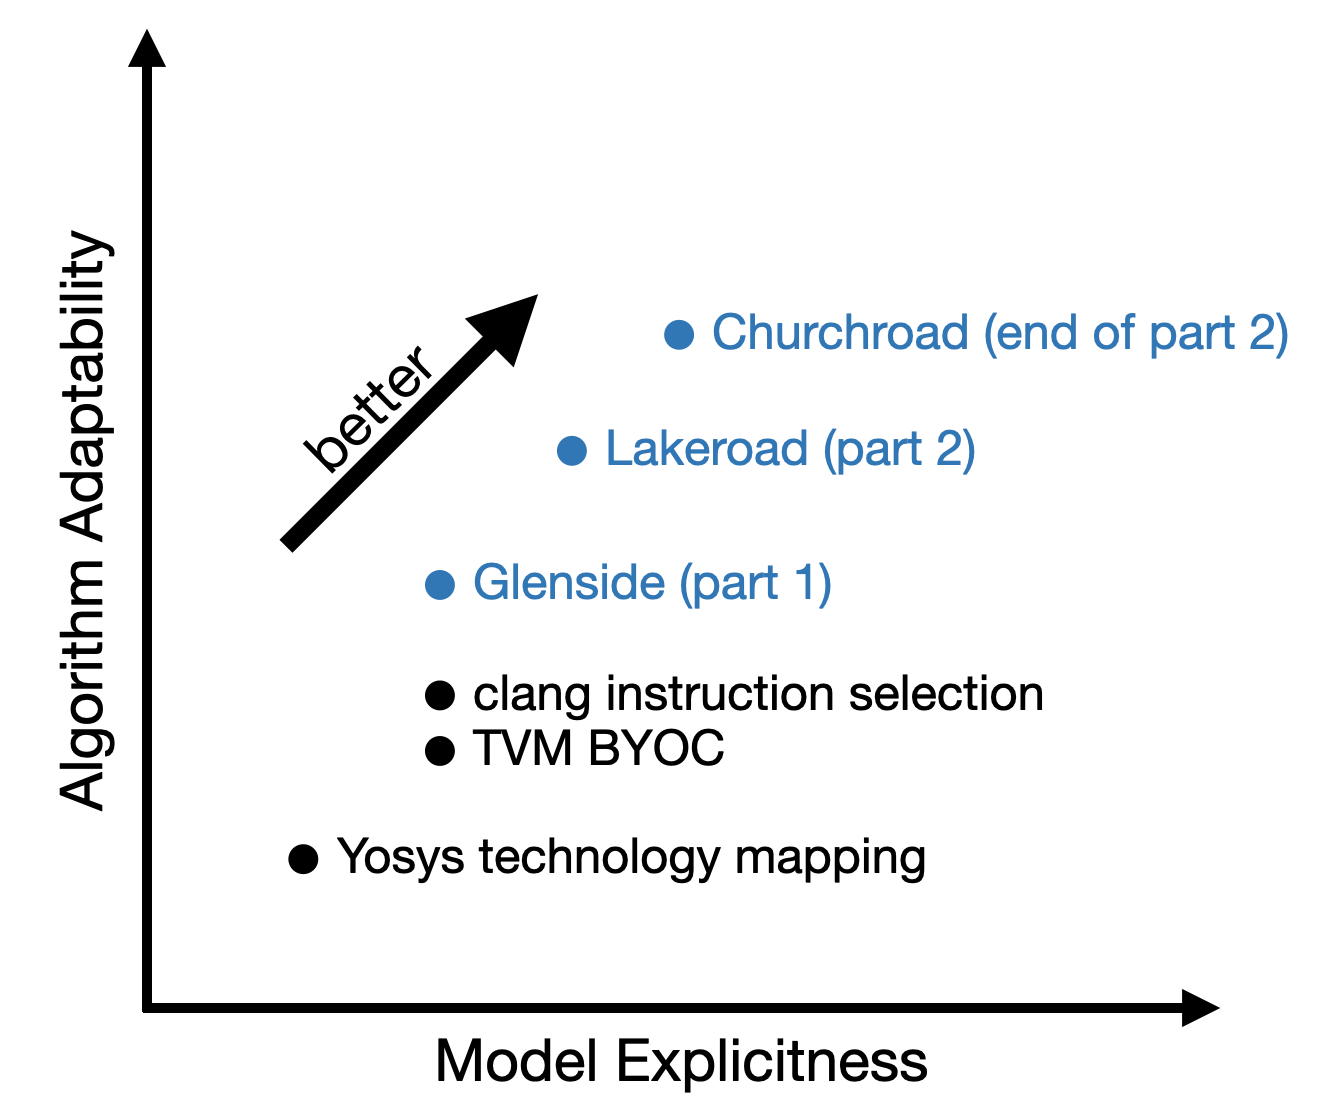
\includegraphics[width=.7\textwidth]{intro-figures/model-alg-spectrum-keynote.png}
    \caption{
A visualization of where various compiler backend
  components
  fall
  on the model explicitness--algorithm automation
  spectrum.
Blue dots represent contributions of this
  dissertation.
    }
    \label{fig:intro:model-alg-spectrum}
\end{figure}



Now that we've introduced these terms,
  let's 
  reconsider the two examples we have discussed so far:
  clang's instruction selector
  and Yosys's technology mapper.
clang's instruction selector is powered by
  an \textit{explicit} model of the x86 ISA,
  part of which is presented in
  \cref{fig:intro:llvm-tablegen}.
Furthermore, its underlying algorithm
  is \textit{adaptable} to new models;
  the user simply needs to update
  the model, and the algorithm will adapt.
On the other hand,
  Yosys's technology mapper utilizes
  \textit{implicit} models,
  and its algorithm is \textit{inflexible}.
To visualize this, we
  we plot Yosys's techology mapper
  and clang's instruction selector
  on a 2D plane
  with model explicitness on the horizontal axis
  and algorithm adaptability on the vertical axis,
  shown in \cref{fig:intro:model-alg-spectrum}.
Yosys's technology mapper,
  being built upon implicit models
  and inflexible algorithms,
  is towards the bottom left.
Meanwhile, clang's instruction selection
  is further up and to the right.

% \hl{move?}
% Note that algorithm adaptability
%   and model explicitness
%   are often intertwined ideas.

\textbf{The core claim of this dissertation,
  put informally,
  is that pushing up
  and to the right
  on our model explicitness--algorithm adaptability
  spectrum (\cref{fig:intro:model-alg-spectrum})
  produces better compiler backends.}
  % that is,
  % using
  % more adaptable algorithms
  % and more explicit models
  % leads to better compiler backends.
By ``pushing up'',
  I mean
  using
  more adaptable
  \gls{automated-reasoning} algorithms
  to automatically generate
  compiler backends
  from explicit, formal models of hardware,
  as opposed to 
  hardcoding backends
  using inflexible algorithms
  and implicit models.
By ``better compiler backends'',
  I focus on three primary classes
  of improvements:
  correctness,
  optimization,
  and development time improvements.
  
Next, I present my formal
  thesis statement.
Afterwards, I will break down the statement
  and discuss each part.

\mdfsetup{
    frametitle={\colorbox{white}{\space{Thesis Statement}\space}},
    innertopmargin=10pt,
    frametitleaboveskip=-9,
    frametitlealignment=\center
    }
\begin{mdframed}
% Defined in toplevel imports-and-macros.tex
\mythesis
\end{mdframed}

\vspace{10mm}

I will now explain and define
  the individual components
  of this thesis.
I will use a set of five keywords
  to refer back to 
  to the primary components of my
  thesis statement:
  its two ``inputs'',
  \cref{thesis:algorithms} and
  \cref{thesis:models},
  and its three ``outputs'',
  \cref{thesis:optimizations},
  \cref{thesis:correctness}, and
  \cref{thesis:devtime}.

\paragraph{Automatically generating compiler 
  backends.}
  \label[thesis:algorithms]{thesis:algorithms}
  \label[thesis:models]{thesis:models}
At the highest level,
  my thesis advocates for
  automatically generating compiler backends.
By this, I mean
  utilizing automated reasoning techniques
  to automatically implement
  compiler backend tasks like
  \gls{tensorization} in ML compilers
  and \gls{technology-mapping} in \gls{fpga} \gls{hardwaresynthesis} tools.
At the highest level,
  automatically generating compiler backends
  takes the form of
  specializing an automated reasoning algorithm
  to a specific compilation task
  by feeding it
  a hardware model.
Thus, I break down the automated generation
  of compiler backends
  into two primary design decisions:
  choosing an automated reasoning algorithm
  (hence referred to with the keyword
    \cref{thesis:algorithms})
  and choosing the formal hardware models
  to feed into the algorithms
  (hence referred to with the keyword
    \cref{thesis:models}).
\cref{thesis:algorithms}
  refers
  to the automated reasoning algorithms
  we use
  to automatically generate our backends.
\cref{thesis:models}
  refers to the hardware models
  which the automated reasoning algorithms
  consume
  to generate the compiler backend.
I thus consider   
  the
  \cref{thesis:algorithms}
  and
  \cref{thesis:models}
  as ``inputs''
  or the independent variables
  in my research.
In \cref{part:glenside-and-3la,part:lakeroad},
  I will show how
  different choices of 
  \cref{thesis:algorithms}
  and
  \cref{thesis:models}
  produce different results.
In
  \cref{part:glenside-and-3la},
  we focus on an algorithm called
  \gls{equality-saturation},
  and
  our models take the form
  of program rewrites
  capturing the high-level 
  functional behavior
  of hardware accelerators.
In
  \cref{part:lakeroad},
  we focus on an algorithm called
  \gls{program-synthesis},
  and
  we directly utilize
  vendor-provided
  Verilog simulation models
  as our models of hardware.

\vspace{10mm}

In my thesis statement,
  I claim that automatically generating
  compiler backends
  benefits compiler
  \cref{thesis:optimizations},
  \cref{thesis:correctness}, and
  \cref{thesis:devtime}.
We consider these the ``outputs''
  or dependent variables
  in our experiments
  in \cref{part:glenside-and-3la,part:lakeroad}.
I now describe each in detail.

\paragraph{\cref{thesis:optimizations}.}
  \label[thesis:optimizations]{thesis:optimizations}
A key task of a compiler backend
  is to utilize the target hardware
  efficiently
  to produce optimized programs.
Compiler backends which rely on poor,
  implicitly encoded models
  and inflexible algorithms
  leave key optimizations on the table.
In \cref{part:glenside-and-3la},
  we demonstrate how inflexible algorithms
  lead to missed accelerator mapping opportunities
  in deep learning compilers.
In \cref{part:lakeroad},
  we show how inflexible algorithms
  and implicit models
  lead to poor utilization
  of specialized FPGA primitives
  during FPGA compilation.
Both of these cases correspond to missed opportunities for optimization.
% \hl{would be nice to show that automated methods have clearly shown
%   to be superior when it comes to optimizing programs.
%   STOKE, AutoTVM, synthesis in general, ML guided?}

\paragraph{\cref{thesis:correctness}.}
  \label[thesis:correctness]{thesis:correctness}
Compiler backends are expected to produce correct code.
However,
  backends which are built on
  implicit models of hardware
  which are deeply integrated into
  the algorithms themselves
  can have hard-to-find bugs.
A cleaner division between hardware model
  and algorithm
  makes it easier to find bugs on either side.
Furthermore, many of the
  more adaptable algorithms
  I advocate for in this dissertation
  (equality saturation, program synthesis)
  have open-source, highly-used, well-tested
  implementations
  which are likely more trustworthy
  than a hand-implemented
  algorithm used only within
  a single compiler backend.
In \cref{part:glenside-and-3la},
  I demonstrate how
  the difficulty of building compilers
  leads to a lack of validation
  in machine learning accelerators.
I show how automatically generating compilers
  for accelerators aids in rapid
  testing and validation,
  and directly leads to uncovering bugs
  in real hardware designs.
In \cref{part:lakeroad},
  I demonstrate how
  utilizing automated reasoning methods,
  we can generate correctness
  guarantees
  stronger than the guarantees
  provided by any
  existing hardware synthesis tool.
  

\paragraph{\cref{thesis:devtime}.}
  \label[thesis:devtime]{thesis:devtime}
And lastly,
  more explicit models
  and more adaptable algorithms
  can ease compiler development.
Implicit models,
  especially models deeply integrated
  into the algorithms themselves
  (such as the Yosys example
    in \cref{fig:intro:yosys-pmgen})
  are generally harder to comprehend
  and thus harder to update.
Understanding implicit,
  imperative models
  is often more challenging
  than understanding explicit,
  declarative models.
More flexible algorithms
  reduce development time in a number of ways.
First, the algorithms
  this dissertation promotes
  all have free-to-use open source 
  implementations,
  thus alleviating the need
  for the compiler engineer
  to write their own algorithm by hand.
Second, the greater flexibility
  of the algorithms
  allows them to adapt to new
  hardware
  with less engineering effort.
In both \cref{part:glenside-and-3la,part:lakeroad},
  we demonstrate
  how compiler backends
  generated with automated reasoning algorithms
  are more easily extensible.
In both cases, to target a new hardware platform,
  users simply need to provide
  models of the target hardware.
In \cref{part:glenside-and-3la},
  these models come in the form of
  rewrites capturing accelerator functionality.
In \cref{part:lakeroad},
  we use simulation models of FPGA primitives
  provided by the FPGA vendors.

\vspace{10mm}

I will demonstrate this thesis
  in two parts.
These parts are visualized on
  our model explicitness--algorithm adaptability
  spectrum in
  \cref{fig:intro:model-alg-spectrum}.
In \cref{part:glenside-and-3la},
  I introduce Glenside~\cite{smith2021pure}
  and \TLA~\cite{huang2024application},
  which demonstrate how
  a more adaptable algorithm
  can increase a compiler's
  ability to offload operations
  to machine learning accelerators.
As is shown in
  \cref{fig:intro:model-alg-spectrum},
  \cref{part:glenside-and-3la}
  only pushes along one axis 
  of our spectrum:
  namely, algorithm adaptability.
In \cref{part:lakeroad}, I
  more fully realize
  my thesis statement
  via Lakeroad~\cite{smith2024fpga}:
  a technology mapper for FPGAs
  which utilizes both more
  adaptable algorithms
  and
  more explicit models.
In the end of \cref{part:lakeroad},
  I also describe Churchroad~\cite{smith2024there},
  which seeks to extend the power of \lr
  to larger hardware designs.
Glenside, Lakeroad, and Churchroad
  demonstrate
  how,
  by automatically generating
  portions of compiler backends
  using more adaptable algorithms
  and more explicit models of hardware,
  we we improve their
  optimization ability and
  correctness, while
  easing development effort.

Before jumping into the content
  of this dissertation, though,
  let me first take the time
  to situate this work
  in the existing literature
  and explain my novel contributions.

\section*{Situating this Dissertation: What's New?}


The automatic generation
  of compilers
  is not a new idea;
  in fact, it has been somewhat
  of a holy grail
  for decades.
So what does this 
  dissertation bring to the table?
Before elaborating on that question,
  I will briefly chronicle
  related work from the past five decades
  related to the top-level topic
  of compiler generation.
Then, I will discuss
  the novel insights of this dissertation:
  namely, 
  (1) taking advantage of the new wave of 
  powerful, off-the-shelf
  automated reasoning tools,
  (2) constraining ourselves
  to domain-specific tasks
  to limit the size of the problem, and
  (3) directly generating
  compiler backends from 
  externally-supplied
  (i.e., not written by us)
  models of hardware.

The earliest citations
  for automated compiler generation
  go back to the late 1960s and early 1970s.
However, 
  though it was often referred to as
  \textit{compiler} generation,
  much of this work focused solely on
  compiler \textit{frontends:}
  parsers and lexers~\cite{
    Newcomer1975MachineindependentGO,
    % peter mosses's phd thesis
    % https://ora.ox.ac.uk/objects/uuid:b590173b-0a86-40c0-8e75-6a6fc5035c43/files/m0e27900b33858b8d881526a8be4b5096
    % generates parsers and lexers from language description
    mosses1975mathematical,
  Jones1980CompilerGF,
  Sethi1981CircularEE,
  Smith2005SemanticsDirectedCG,
  Feldman1968TranslatorWS}.
A common task was,
  given a grammar for a new programming language,
  could you generate the parser and lexer
  for that language.
This work culminated in 
  industry-standard tools
  like Yacc and GNU Bison.
Even just Yacc's name, which stands for
  ``yet another compiler--compiler''
  shows how our terminology may have changed;
  while Yacc might have been considered
  a compiler--compiler in the past,
  now it only handles the very frontend
  of compiler tasks: the parser and lexer.

However, not all of the initial wave of research
  focused on compiler frontends.
There was also work on generating components
  of compiler \textit{backends}---%
  often referred to as 
  ``code generation.''
In a 1977 survey of code generators 
  from R.~G.~Cattell~\cite{cattell1977survey},
  he states:
  \begin{quote}
Traditionally, compiler-generation systems have
been weak on automating the later stages of compilation, specifically code generation.
But as the formal methods and grammars applied have become better understood and
more powerful, their scope has gradually been evolving towards the later stages of
compilation.
  \end{quote}
Certainly this entire dissertation
  can simply be seen as one more step
  in this gradual evolution.
As we will discuss later,
  this dissertation benefits from
  the nearly five decades
  of formal methods and automated reasoning research
  since the time of Cattell's writing.

Nonetheless,
  researchers did approach the topic
  of backend generation~\cite{
  snyder1975portable,
  fraser1988automatic}.
Interestingly,
  the spectrum I identify
  earlier in this chapter---%
  the model explicitness--algorithm adaptability spectrum---%
  seems to apply even in the early years
  of automated backend generation research.
% https://apps.dtic.mil/sti/tr/pdf/ADA056027.pdf
In his 1977 survey, Cattell
  describes a very similar spectrum
  in methods of 
  automatically producing code generators:
\begin{quote}
In general, there have been two kinds of approaches to more automatic production of
code generators. The first is the development of a specialized language for code
generators, with built-in machinery for dealing with common details of the process.
The second extreme is the development of a program to build a code generator for a
language from a purely structural and behavioral machine description. Rather than
being mutually exclusive, these procedural and descriptive language approaches,
respectively, represent points in a continuum of degrees of automatic programming.
\end{quote}
The two extremes on Cattell's spectrum
  have analogous points on my
  model explicitness--algorithm adaptability spectrum.
At one extreme
  on his spectrum,
  he is essentially describing
  code generator \glspl{dsl}:
  specialized languages for
  building procedural (in his words)
  or imperative (in mine)
  code generators.
We've already seen a
  modern example of this---%
  Yosys's pmgen DSL
  in \cref{fig:intro:yosys-pmgen}.
At the other extreme of his spectrum
  are programs which produce code generators from
  descriptive/structural (in his words)
  or declarative (in mine)
  machine descriptions and hardware models.
Again, we have seen a modern example of this
  in \cref{fig:intro:llvm-tablegen}: 
  clang's instruction selector
  and the declarative model of the ISA
  which it consumes.
  


% From Cattell's [PDF] A survey and critique of some models of code generation
% There is a comparatively long history of compiler-writing systems, dealing with codegeneration to lesser or greater extents. These efforts have all taken the specialized
% language approach. An early example is Feldman [1966], who uses a language FSL for
% description of programming language semantics (code generation). In combination with
% a syntax description, it was used in a compiler-compiler. It was somewhat primitive,
% but did deal with errors, forward references, and simple storage allocation. Feldman
% and Gries [1968 ] and McKeeman et al [1970] survey more advanced translator writing
% systems. More recently, White [1973] and Ganzinger et al [1977 ] describe compilergeneration systems along this line. Traditionally, compiler-generation systems have
% been weak on automating the later stages of compilation, specifically code generation.
% But as the formal methods and grammars applied have become better understood and
% more powerful, their scope has gradually been evolving towards the later stages of
% compilation. 
%
% This paper has an insanely helpful table near the end.
% Things to look into basedd on the table:

Much of the early work on
  the automated generation of code generators
  (i.e.~compiler backends)
  was based on intermediate representations.
To generate compilers,
  these works introduce an intermediate
  representation;
  then, those wishing to generate a compiler
  would then specify how to compile
  that intermediate representation
  to their target machine.
A prime example of this 
  was Perry Miller's DMACS system~\cite{miller1971automatic}
  where DMACS stood for
  ``Descriptive MACro code generating System.''
This
  system introduced
  macros, which were 
  machine-independent
  operations
  which could be implemented
  differently
  for each target machine.
Much of this work can be seen
  as the predecessors
  of the 
  now-standard method of building compilers
  using one or a number of
  intermediate representations,
  most recently made popular
  by the
  foundational LLVM compiler 
  toolchain~\cite{lattner2004llvm}.

While it is further
  from the work of this dissertation,
  it is also worth mentioning work on
  partial evaluation~\cite{consel1993tutorial,futamura1999partial}.
Futamura projections
  specifically
  are of interest,
  as they describe how compilers can
  be viewed as partial evaluations
  of interpreters.
I do not use any partial evaluation techniques
  in this dissertation.

% \hl{
% Donegan 1973 An Approach to the Autonio.tic Generation of Cod. Cen.rtuors
% }

% \hl{
% Weingart 1973 An Eff icient and Systematic Method of Compiler Cod. Generat ion
% }

% \hl{
% Newcomer 1975 : Machine Independent Generation of Optimal Local Code
% }


%https://www.semanticscholar.org/paper/Survey-on-Instruction-Selection%3A-An-Extensive-and-Blindell/628a73a92c6112c3b4651cf2d940a5ba51590f21
% \hl{
% survey on instruction selection
% }

%https://www.semanticscholar.org/paper/A-truly-generative-semantics-directed-compiler-Ganzinger-Giegerich/ec945309806c3090f6da62d8063d953b3fecfea9
% \hl{Ganzinger's work.}
% The MUG2 system~\cite{Ganzinger1982ATG,Ganzinger1977AutomaticGO}
%   is a so-called ``compiler compiler'', 
%   which takes 

% https://apps.dtic.mil/sti/pdfs/ADA019571.pdf
% \cite{Newcomer1975MachineindependentGO}
% As he puts it,
% ``There has been extensive research into the automatic generation of compilers.
% Much of this has concentrated on the issues of syntax and semantics, while little has
% been done on the problems of code generation.''
% He states
%   how efficiency has been mostly ignored
%   when considering portability;
%   that is, if someone came up with a system to port code
%   from one system to another,
%   they'd be satisfied,
%   regardless of how good the port was.
% He argues we need to pay more attention to 
%   producing efficient code.
% You can potentially simplify that argument:
%   we shouldn't always assume
%   translators are available in the first place.
% Especially once you begin considering
%   the broad range of targets which exist
%   at the backend of a compiler, especially
%   now.
% If they were just considering 
%   general-purpose processors back then,
%   then maybe retargeting was reasonable.


In the ensuing five decades,
  the topic of automated backend
  generation
  has seen steady interest~\cite{
  buchwald2018synthesizing,
  dias2010automatically,
  brandner2007compiler,
  daly2022synthesizing,
  leupers1997retargetable,
  brandner2013automatic}.
In the next few paragraphs,
  I highlight notable trends
  and important projects.
  
A common pattern in recent research
  is the application
  of more and more powerful
  \gls{automated-reasoning} algorithms,
  especially those employed in this dissertation:
  term rewriting~\cite{Richards2006VerificationOC,Despland1990UsingRT,Emmelmann1991CodeSB,Despland1990PAGODEAB,Daly2024EfficientlySL} and 
  synthesis based on \gls{smt}~\cite{Daly2024EfficientlySL}.
% Spiral
One of the most notable projects
  in this space
  is SPIRAL~\cite{franchetti2018spiral}. 
Historically,
  SPIRAL is an umbrella
  over many related grants,
  researchers, and projects,
  but at its core is the
  SPIRAL compiler.
The SPIRAL compiler's goal
  is to enable performance
  portability
  of specialized kernels
  across a wide range of architectures.
They use many techniques
  also used in this dissertation,
  such as
  capturing programs in a high-level,
  backend-nonspecific language
  and
  utilizing automated reasoning 
  (in their case, term rewriting systems)
  to adapt their compiler
  to different backends.


% Norman Ramsey
Another point worthy of note
  is the work of Norman Ramsey
  and his student Jo\~{a}o Dias,
  whose work on generating
  instruction selectors
  (among other compiler components)
  is very reminiscent
  of the work in this dissertation~\cite{
  ramsey2003pragmatic,
  ramsey2011resourceable,
  dias2010automatically}.
As is the general pattern
  in the work in this area,
  Ramsey and Dias
  focus on utilizing automated reasoning algorithms
  and high-level machine descriptions
  to implement compiler backend components,
  saving compiler development time.


If this dissertation focuses on
  generating software (i.e.~compilers)
  from hardware,
  it is important to also mention
  the parallel line of research
  which attempts to generate hardware from software.
Programs are a literal description
  of what needs to be computed;
  why not use them to determine
  what hardware we should make?
A perfect example of this is
  the concept of \gls{hls}~\cite{cong2011high,cong2022fpga}
  which allows hardware designers to produce hardware
  from
  software algorithms
  written in high-level languages like C.\footnote{
Note that the reality of modern HLS
  is a little messier than described,
  but this is the intention.
}
There is also an entire literature on
  hardware--software codesign~\cite{teich2012hardware,kokila2016survey,schaumont2012practical,wolf2003decade,Gupta1993HardwaresoftwareCF},
  which, while rich and varied,
  generally centers on the idea
  of exploring the hardware design space
  using representative software workloads
  as a starting place.
In fact,
  \g (presented in \cref{part:glenside-and-3la})
  was originally a
  hardware--software codesign tool
  which aimed to use equality saturation
  to rewrite machine learning models
  into potential accelerator designs.

The ideas presented in this dissertation
  are complementary
  to the ideas of hardware--software codesign,
  and
  I believe we should pursue both directions.
The core idea presented in
  this dissertation---%
  generating compiler backends
  from formal models of hardware---%
  targets the lower layers of the compiler stack.
In general, this dissertation answers the question of,
  given low-level primitives,
  how do we find places 
  to use those primitives 
  in programs or hardware designs?
Hardware--software codesign, on the other hand,
  targets higher levels of the stack.
Codesign seeks to answer the question,
  what hardware \textit{should} we design,
  given the software we need to run?
Thus, the methods presented here
  will only benefit codesign;
  better technology mapping from \lr, for example,
  will only benefit the designs
  produced by HLS tools.
  


I claim there are three specific features
  of this dissertation
  which set it apart from existing literature.
First is our focus on
  using
  \textit{off-the-shelf}
  automated reasoning tools,
  rather than developing our own.
Second is constraining ourselves
  to domain-specific tasks
  to limit the size of the 
  generation problem.
And last is the generation of
  compiler backends from 
  \textit{externally-supplied}
  (i.e., not written by us)
  models of hardware.
I will now discuss each of these in detail.

First, since the inception of
  automated compiler backend generation
  as a research topic,
  there have been significant
  advances in
  \gls{automated-reasoning} techniques,
  e.g.~%
  % languages and type systems
  % for hardware~\cite{durst2020type,nigam2023modular,nigam2020predictable},
  equational reasoning via \gls{equality-saturation}~\cite{tate2009equality,willsey2021egg},
  \gls{program-synthesis}~\cite{solar2008program,torlak2013growing},
  and machine learning for program generation~\cite{alon2019code2vec,austin2021program}.
Many of these advances
  have made automated reasoning techniques
  accessible to a broader audience.
Whereas previous work
  often may need to build 
  automated reasoning techniques
  by hand,
  in this dissertation I show how
  off-the-shelf tools
  have become powerful enough
  to use for tasks of this magnitude.
Specifically, I utilize
  the
  equality saturation
  library \texttt{egg}~\cite{willsey2021egg}
  in \cref{part:glenside-and-3la}
  and the program synthesis library
  Rosette~\cite{
  torlak2013growing,torlak2014lightweight}
  in \cref{part:lakeroad}.
  
  

Second, we focus on
  compiler generation
  for specialized hardware backends.
Compiler backend generation projects
  of the past often focused on
  generating compiler components
  for general-purpose processors~\cite{
  fauth1995describing,
  leupers1997retargetable,
  brandner2007compiler,
  brandner2009automatic,
  brandner2013automatic,
  ramsey2003pragmatic,
  ramsey2011resourceable,
  dias2010automatically}.
As hardware becomes more heterogeneous,
  however,
  the variety of hardware targets
  needing compilers
  has increased.
In this dissertation,
  we focus instead on 
  building compiler components
  for new, specialized platforms---%
  machine learning accelerators
  in \cref{part:glenside-and-3la}
  and specialized \gls{fpga} \glspl{primitive}
  like DSPs in
  \cref{part:lakeroad}.
Not only are compilers
  needed for these new specialized targets,
  but their specialization
  also constrains the search space,
  making automated reasoning
  far more tractable.


Lastly,
  while previous works have often leaned
  on machine descriptions~\cite{
  ramsey2011resourceable}
  when generating compiler components,
  these machine descriptions
  generally must be handwritten
  by the compiler engineer
  utilizing the compiler generation
  framework.
In \cref{part:lakeroad}
  we introduce a new technique---%
  semantics extraction from Verilog---%
  which directly leverages vendor-supplied
  Verilog.
Many of these models are
  built to be used with
  automated reasoning tools,
  but are currently only utilized for
  \textit{post-compilation verification,}
  rather than in compilation itself~\cite{sisco2022position,sisco2022synthesis}.
I demonstrate how these models
  can be used
  to generate more correct, more complete compilers
  for specialized hardware.

